\documentclass[a4paper,14pt]{extarticle}

\usepackage[utf8x]{inputenc}
\usepackage[T1,T2A]{fontenc}
\usepackage[russian]{babel}
\usepackage{hyperref}
\usepackage{indentfirst}
\usepackage{here}
\usepackage{array}
\usepackage{graphicx}
\usepackage{caption}
\usepackage{subcaption}
\usepackage{chngcntr}
\usepackage{amsmath}
\usepackage{amssymb}
\usepackage{pgfplots}
\usepackage{pgfplotstable}
\usepackage[left=2cm,right=2cm,top=2cm,bottom=2cm,bindingoffset=0cm]{geometry}
\usepackage{multicol}
\usepackage{askmaps}
\usepackage{titlesec}
\usepackage{listings}
\usepackage{color}
\usepackage{courier}

\definecolor{green}{rgb}{0,0.6,0}
\definecolor{gray}{rgb}{0.5,0.5,0.5}
\definecolor{purple}{rgb}{0.58,0,0.82}

\lstset{
	language=Verilog,
	backgroundcolor=\color{white},   
	basicstyle=\small\ttfamily,
	commentstyle=\color{green},
	keywordstyle=\color{blue},	
	numberstyle=\tiny\color{gray},
	stringstyle=\color{purple},
	breakatwhitespace=false,
	breaklines=true,
	captionpos=b,
	keepspaces=true,
	numbers=left,
	numbersep=5pt,
	showspaces=false,
	showstringspaces=false,
	showtabs=false,
	tabsize=4,
	frame=single,
	inputpath={../quartus/},
	literate={~} {$\sim$}{1}
}

\renewcommand{\le}{\ensuremath{\leqslant}}
\renewcommand{\leq}{\ensuremath{\leqslant}}
\renewcommand{\ge}{\ensuremath{\geqslant}}
\renewcommand{\geq}{\ensuremath{\geqslant}}
\renewcommand{\epsilon}{\ensuremath{\varepsilon}}
\renewcommand{\phi}{\ensuremath{\varphi}}
\renewcommand{\thefigure}{\arabic{figure}} 	
\renewcommand*\not[1]{\overline{#1}}

\titleformat*{\section}{\large\bfseries} 
\titleformat*{\subsection}{\normalsize\bfseries} 
\titleformat*{\subsubsection}{\normalsize\bfseries} 
\titleformat*{\paragraph}{\normalsize\bfseries} 
\titleformat*{\subparagraph}{\normalsize\bfseries} 

\counterwithin{figure}{section}
\counterwithin{equation}{section}
\counterwithin{table}{section}
\newcommand{\sign}[1][5cm]{\makebox[#1]{\hrulefill}}
\graphicspath{{../pics/}}
\captionsetup{justification=centering,margin=1cm}
\def\arraystretch{1.3}
\setlength\parindent{5ex}
\titlelabel{\thetitle.\quad}

\begin{document}

\begin{titlepage}
\begin{center}
	Санкт-Петербургский Политехнический Университет Петра Великого\\[0.3cm]
	Институт компьютерных наук и технологий \\[0.3cm]
	Кафедра компьютерных систем и программных технологий\\[4cm]
	
	\textbf{ОТЧЕТ}\\ 
	\textbf{по лабораторной работе}\\[0.5cm]
	\textbf{SystemVerilog №4}\\[0.1cm]
	Автоматизация проектирования\\ дискретных устройств\\[4.0cm]
\end{center}

\begin{flushright}
	\begin{minipage}{0.45\textwidth}
		\textbf{Работу выполнил студент}\\[3mm]
		группа 33501/4 \hspace*{9mm} Дьячков В.В.\\[5mm]
		\textbf{Преподаватель}\\[5mm]
		\sign[1.5cm] \hspace*{1mm} к.т.н., доц. Филиппов А.С. \\[5mm]
	\end{minipage}
\end{flushright}

\vfill

\begin{center}
	Санкт-Петербург\\
	\the\year
\end{center}
\end{titlepage}

\addtocounter{page}{1}
\counterwithin{lstlisting}{section}

\tableofcontents
\lstlistoflistings
\listoffigures
\newpage

\section{Введение}

Устройство передачи данных решает три укрупненных задачи:
\begin{enumerate}
	\item Прием и буферизация данных от нескольких источников синхронных сигналов (синхросигнал расположен фронтом по центру бита, фазовый разброс $\pm1$ нс). Поток входных данных идет непрерывно.
	\item Когда в буфере FIFO накапливаются данные, достаточные для формирования пакета, устройство управления выдает команду блоку коммутации и формирования пакета, который формирует пакет в соответствии с заданием. Если данные для передачи отсутствуют, передается "пустой" пакет с отсутствующими данными, $M=0$ по каналу $N=15$.
	\item LVDS Transmitter - передатчик LVDS канала обеспечивает передачу синхронных дифференциальных данных по заданному числу каналов (Number of Channals) с заданной скоростью передачи (Output data rate).
\end{enumerate}

На рис. \ref{fig:structure} приведена укрупненная структурная схема устройства передачи данных.
\begin{figure}[H]
	\centering
	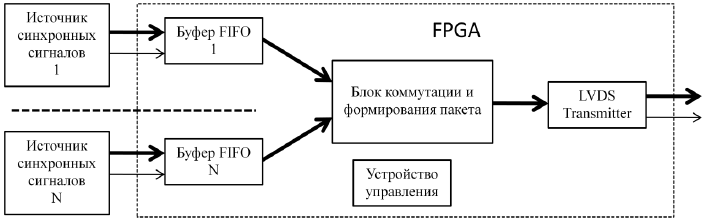
\includegraphics[width=\linewidth]{structure}
	\caption{Укрупненная структурная схема устройства}
	\label{fig:structure}
\end{figure}

\section{Исходные данные}

\begin{itemize}
	\item Три 16-разрядных источника сигналов, частота 10 МГц;
	\item Количество байт данных $M = 9$;
	\item Формат пакета: \code{H1MD} (\code{H1} -- первый байт заголовка \code{0xFN}, \code{M} -- количество байт данных, \code{D} -- передаваемые данные);
 	\item Двухканальный LVDS передатчик, скорость передачи данных $600$ Мб/с.
\end{itemize}

\section{Анализ технического задания}

\begin{itemize}
	\item Анализ вариантов реализации и разработка структурной семы устройства.
	\item Детализация структурных блоков, разработка функциональной схемы устройства.
	\item Анализ IP-функций, используемых в устройстве, формирование требований к разрабатываемым блокам.
		\begin{itemize}
			\item \code{FIFO}
			\item \code{ALTLVDS_TX}
		\end{itemize}
\end{itemize}

\section{Разработка функционально-логического описания и моделирование}

\begin{itemize}
	\item Организация FIFO.
	\item Организация и настройка передатчика LVDS.
	\item Разработка блока коммутации.
	\item Разработка устройства управления.
	\item Интеграция разработанных блоков и моделирование работы устройства передачи данных.
\end{itemize}

\section{Верификация устройства передачи данных в системном окружении}

\begin{itemize}
	\item Разработка имитатора системного окружения, задающего поток входных данных.
	\item Создание и настройка средств системной отладки.
	\item Исследование работы устройства передачи данных на плате-прототипе (Mini DiLab).
\end{itemize}

\section{Заключение}

\end{document}